\documentclass[border=5mm]{standalone}
\usepackage{tikz}
\usetikzlibrary{arrows.meta, intersections}

\begin{document}

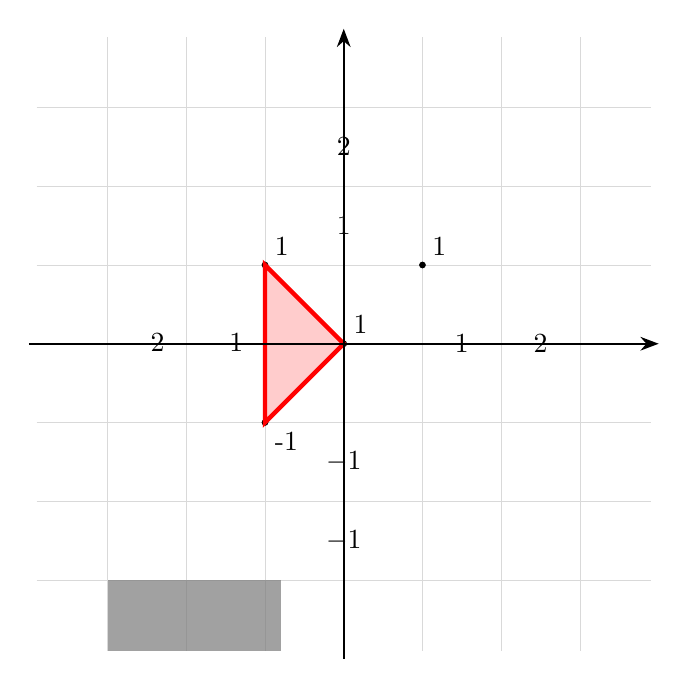
\begin{tikzpicture}[scale=1]
    % Draw grid with light gray color
    \draw[help lines, color=gray!30] (-3.9,-3.9) grid (3.9,3.9);
    
    % Plot the vertices of the polygon
    \filldraw [black] (0,0) circle (1pt);
    \filldraw [black] (-1,1) circle (1pt);
    \filldraw [black] (-1,-1) circle (1pt);
    \filldraw [black] (1,1) circle (1pt);
    
    % Draw the edges of the polygon
    \draw[ultra thick, red, name path=poly1] 
        (0,0) -- 
        (-1,1) -- 
        (-1,-1) -- 
        (0,0) -- cycle;
    
    % Draw the apexes of the polygon
    \node at (0,0) [above right] {1};
    \node at (-1,1) [above right] {1};
    \node at (-1,-1) [below right] {-1};
    \node at (1,1) [above right] {1};
    
    % Draw the region in red
    \fill [red, opacity=0.2] (0,0) -- (-1,1) -- (-1,-1) -- cycle;
    
    % Draw the regions in gray
    \fill [gray, opacity=0.2] (-3,-3) rectangle (-0.8,-3.9);
    \fill [gray, opacity=0.2] (-3,-3) rectangle (-0.8,-3.9);
    \fill [gray, opacity=0.2] (-3,-3) rectangle (-0.8,-3.9);
    \fill [gray, opacity=0.2] (-3,-3) rectangle (-0.8,-3.9);
    \fill [gray, opacity=0.2] (-3,-3) rectangle (-0.8,-3.9);
    \fill [gray, opacity=0.2] (-3,-3) rectangle (-0.8,-3.9);
    
    % Draw the axes
    \draw[-Stealth, thick] (-4,0) -- (4,0); % x-axis
    \draw[-Stealth, thick] (0,-4) -- (0,4); % y-axis
    
    % Label axes
    \node at (-2.5,0) {$-2$};
    \node at (-1.5,0) {$-1$};
    \node at (1.5,0) {$1$};
    \node at (2.5,0) {$2$};
    
    \node at (0,-2.5) {$-1$};
    \node at (0,-1.5) {$-1$};
    \node at (0,1.5) {$1$};
    \node at (0,2.5) {$2$};
    
\end{tikzpicture}

\end{document}